\chapter{メールの通信の保護}

メールデータをやりと利すとき、その通信経路としてインターネットを使います。
本章では、インターネットを開催多サーバ接続のセキュリティについて取り上げます。

SMTPは、成立年代が古いこともあり、現在でも平文で通信が行われることが多いプロトコルです。
ですが、TLSによる接続先の確認と、通信の暗号化を図ることが可能です

では、その経路で、メールの通信を保護するセキュリティとはどのようなものなのでしょうか。

\section{TLSを使用した通信}

メールの通信を保護するには、経路となるインターネットの上で流れる通信を暗号化するのが一般的なやり方です。
では、データの暗号化による経路保護とはどのように行うのでしょうか。本章は、それについて解説をします。

\subsection{TLSの利用}

結論からいけば、メールの通信の経路暗号化は、TLSによっておこないます。
一般的には、SSL/TLSとして扱われることがありますが、本書ではTLSという表記で統一します。

メールに関する通信は、大きく三種類に分類することができます。
メールサーバとメールサーあの間のメール転送、メール送信時の、クライアントからメールサーバへの通信。
この二種は、SMTPによって行われます。

最後のひとつは、メールサーバに蓄積されたメールデータにクライアントが隠せすする通信です。これは、POP3もしくはIMAPが用いられます。

これらの通信は、全てTCPをトランスポート層として行われる、アプリケーション層の通信です。
TCPを使うということは、暗号化レイヤとしてTLSを挟むことができるということでもあります。

現在の多くのMTAやMRAの実装で、通信の暗号化レイヤとして、TLSを利用できるようになっています。

\subsection{二つのTLS利用方式}

SMTPでTLSを利用する場合、暗黙的なTLSと、明示的なTLSの二つの利用形態があります。これはSMTPやPOP3,IMAPといったメールに関連するプロトコルに限ったことではないのですが、それについて説明をしましょう。

\subsubsection{暗黙的なTLS}

\begin{figure}[htbp]
	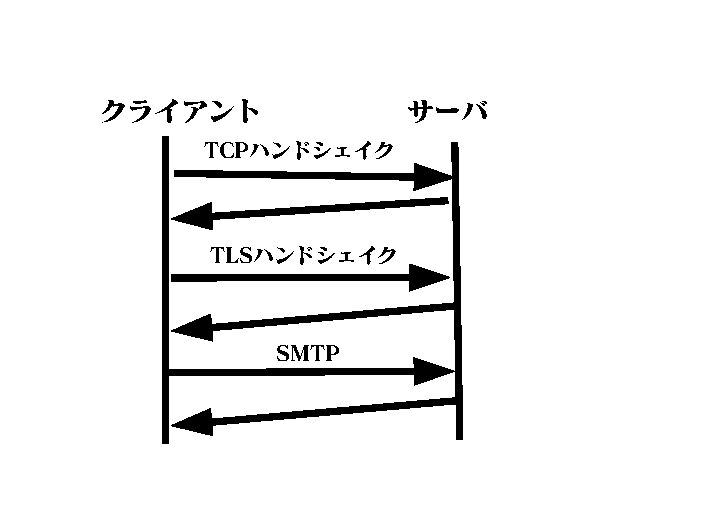
\includegraphics[width=12cm,clip]{draw/implicit.pdf}
	\caption{暗黙的TLS}
	\label{fig:implicit_TLS}
\end{figure}

暗黙的なTLS(Implicit TLS)とは、アプリケーション層の通信はTLSで暗号化することを前提にして、TCPのハンドシェイク後、アプリケーションの通信が始まる前にTLSのハンドシェイクを行います。
その後、アプリケーションの通信は、TLSで暗号化された経路の上で行われます。
この流れを図示すると、図\ref{fig:implicit_TLS}のようになります。

このように、暗黙のうちにTLSのハンドシェイクが行われ、その上でアプリケーションの通信顔こなれることから、この方式を暗黙的TLSといいます。

暗黙的TLSを用いる通信は、TLSを用いない、オリジナルの通信とは別のポートを使うという特徴があります。代表的なものはHTTPと、暗黙的TLSを用いるHTTPSで、それぞれ、Well-Knownポートは80/TCPと443/TCPです。

暗黙的TLSの場合は、オリジナルのプロトコルの名前の末尾に大文字のSを付けて表記します。このSは、TLSの前身となったSSLに由来します。
読み下すときは、over SSLもしくはover TLSと読みます。

メール関連のプロトコルで暗黙的なTLSを使用する場合は、以下のようにプロトコル名称と使用するポートを変更します。

\begin{table}[htb]
  \begin{tabular}{lrlr} \hline
    プロトコル & ポート & TLS使用時名称 & TLS使用時ポート \\ \hline \hline
    SMTP & 25/TCP & SMTPS & 465/TCP \\
    POP3 & 110/TCP & POP3S & 995/TCP \\
    IMAP & 143/TCP & IMAPs & 993/TCP \\ \hline
  \end{tabular}
\end{table}

ただし、SMTPSは後述するSMTP-AUTHでクライアント認証を行う用途に使われるため、サーバ間の転送では使用されません。

\subsection{明示的なTLS}

\begin{figure}[htbp]
	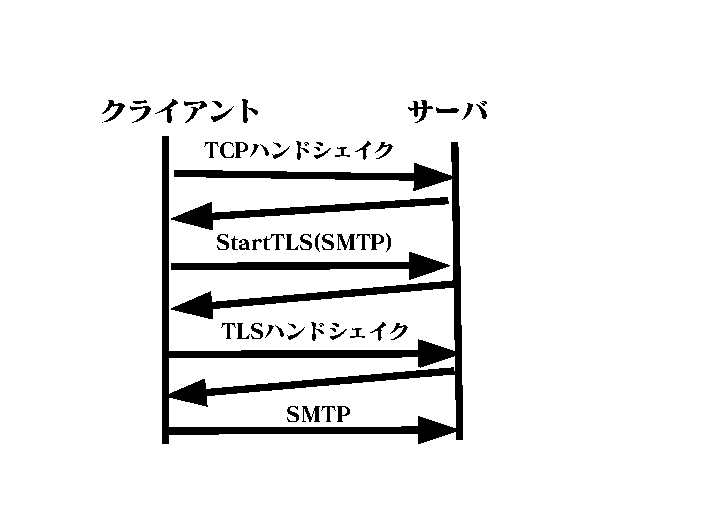
\includegraphics[width=12cm,clip]{draw/explicit.pdf}
	\caption{明示的TLS}
	\label{fig:explicit_TLS}
\end{figure}

明示的なTLS(Explicit TLS)とは、TCPのセッションが始まってから、アプリケーション層の通信で、TLSの通信を開始するネゴシエーションを行います。

この場合、TCPのネゴシエーションが終わったら、平文でプロトコルのアプrケーション層のセッションを始めます。
その中で、TLSを使用するかのネゴシエーションを行い、双方が合意したら、TLSのネゴシエーションを行います。
TLSのネゴシエーションも、TCPから見れば上位レイヤーの通信であるため、実装で対応する限り、成立したTCPセッションの中で、どのタイミングからでも始めることができます。

この流れを図示すると、図\ref{fig:explicit_TLS}になります。

TLSを使用するかの問い合わせは、アプリケーション層のSTARTTLSというコマンドを送信します。そのため、明示的なTLSを使用する通信であることを明示するときは、プロトコル名のあとに、with StartTLSと記載することがあります。

このような手順を取る理由は、通信に置いてTLSを使用しないという選択をするためです。そのため、StartTLSを使用する場合は、元のプロトコルと同じポートを通信に使用します。
たとえば、SMTP with StartTLSの場合は、25/TCPを使用します。同様に、POP3 with StartTLSは110/TCPを、IMAP with StartTLSは、143/TCPを使用します。

また、後述するSMTP-AUTHでクライアント認証を行う場合、クライアントとメールサーバの間のアプリケーション層プロトコルはSMTPですが、587/TCPを用います。

\section{通信の保護のための証明書}

ここまで背つめしたいように、メールに関連するプロトコルでも、TLSを使用することができます。
TLSであるということは、証明書が必要になります。
この証明書は、どのようなものなのでしょうあk。

メールで使用する証明書は、一般的なTLSの証明書です。
Webサーバで使用する証明書と同じ種類のものとなります。
そのため、必要なレベルの証明書を、証明局に発行してもらうという、サーバ証明書発行の手順となります。

\subsection{自家証明書}

TLSの証明書とは、公開鍵暗号の、公開鍵に電子署名をしたものです。、
証明局とよばれる機関にひょる電子署名が必要です。証明書の正当性は、この電子署名によって行われます。これが、証明局が証明書を発行するということの正体です。

証明局は、発行を依頼する個人、団体の正当性を確認した上で、署名を行います。
つまり、TLSの証明書には、暗号化の鍵とは別に、第三者によって、所有者が認証されていることで正当性を示す、という機能があります。

この証明局による証明は、費用が発生します。そのため、試験段階など、電子署名も自分で行った、非正規の証明書を使うことがあります。この、証明局による署名を経ていない証明書を、自家署名証明書、あるいは、自家証明書と呼びます。
俗に、オレオレ証明書、と呼ばれることもあります。

自家証明書は、公開鍵であるため暗号化に使用することはできます。ですが、認証局による署名がされていないため、サーバと、証明書そのものの正当性を示すことができません。そのため、メール関連の通信を保護する目的であっても、自家証明書は使用すべきではありません。

\subsection{証明書の確認}

SMTPで証明書を使用するとしたら、それは経路の暗号化もですが、通信相手のサーバの正当性を確認することも目的となります。
そのため、サーバ間通信のための証明書は、自家署名でない正当なものを使用すべきです。
また、接続先が自家署名の証明書を使用している場合や、サーバ名と証明書の名前が一致しない場合は、接続を拒否する設定が、セキュリティ的に推奨されます。



\section{TLSでなにを保護するか}

ここまでで、メールに関連するプロトコルでTLSを使用する場合についての説明を行いました。
では、TLSで何を保護するのでしょうか。

\subsection{サーバ間の通信}

メールサービスでサーバ間の通信は、SMTPによるメール転送です。
正確を期すると、SMPTはクライアント・サーバ型のプロトコルです。
ですが、ここでは、メールサーバとメールサーバの間の通信という意味で、サーバ間の通信というように記載します。
この通信をTLSで保護する場合、それはメールデータの暗号化による保護という綿もありますが、通信相手のサーバの正当性を確認するという用途もあります。

サーバとサーバの通信では、SMTP with StartTLSを用います。これは、SMTPSで使用する465/TCPは、一般的に、SASLによるユーザ認証を設定して、そのメールサーバのユーザがメールを送信するのに使用することが多いためです。

ただし、2019年現在で、サーバ間通信でSMTP with StartTLSに対応しているサーバは多くありません。
そのため、TLSの使用を選択できるTartTLSを用いることと、TLSの利用を必須としない設定にするほうが無難ということになります。


\subsection{クライアントとサーバの間の通信}

メールサービスで、クライアントとサーバの間の通信をTLSで保護する場合、それは何を保護するのでしょうか。

メールのエコシステムにおいて、クライアント・サーバ型の通信になるのは、メールクライアントソフトからメールサーバにSMTPで接続して、メールを転送する場合があります。
もうひとつは、POP3もしくはIMAPで、受信メールを蓄積しているサーバに接続する場合です。

これらの通信にTLSを適用する場合、その目的は主に、通信の暗号化となります。
クライアントからサーバへの通信は、多くの場合、ユーザ認証をともないます。

SMTPでサーバにメールを転送する際は、認証フレームワークのSASLを用いて、ユーザ認証を行います。
そして、認証されたユーザからのメール転送を受け付けます。

POP3やIMAPでメールデータを蓄積するサーバに接続する場合は、そのプロトコルに組み込まれたユーザ認証をもちいて、認証されたユーザに対応するメールデータへのアクセスが可能となります。
この時もユーザアカウントとパスワード、もしくはパスワードを暗号化した情報を通信するので、TLSでその通信を保護します。


